\newgeometry{
    margin=1.5cm,
    noheadfoot, nomarginpar,
    footskip=1.25em,
}

\begin{landscape}
\begin{figure}[!ht]
    \centering
    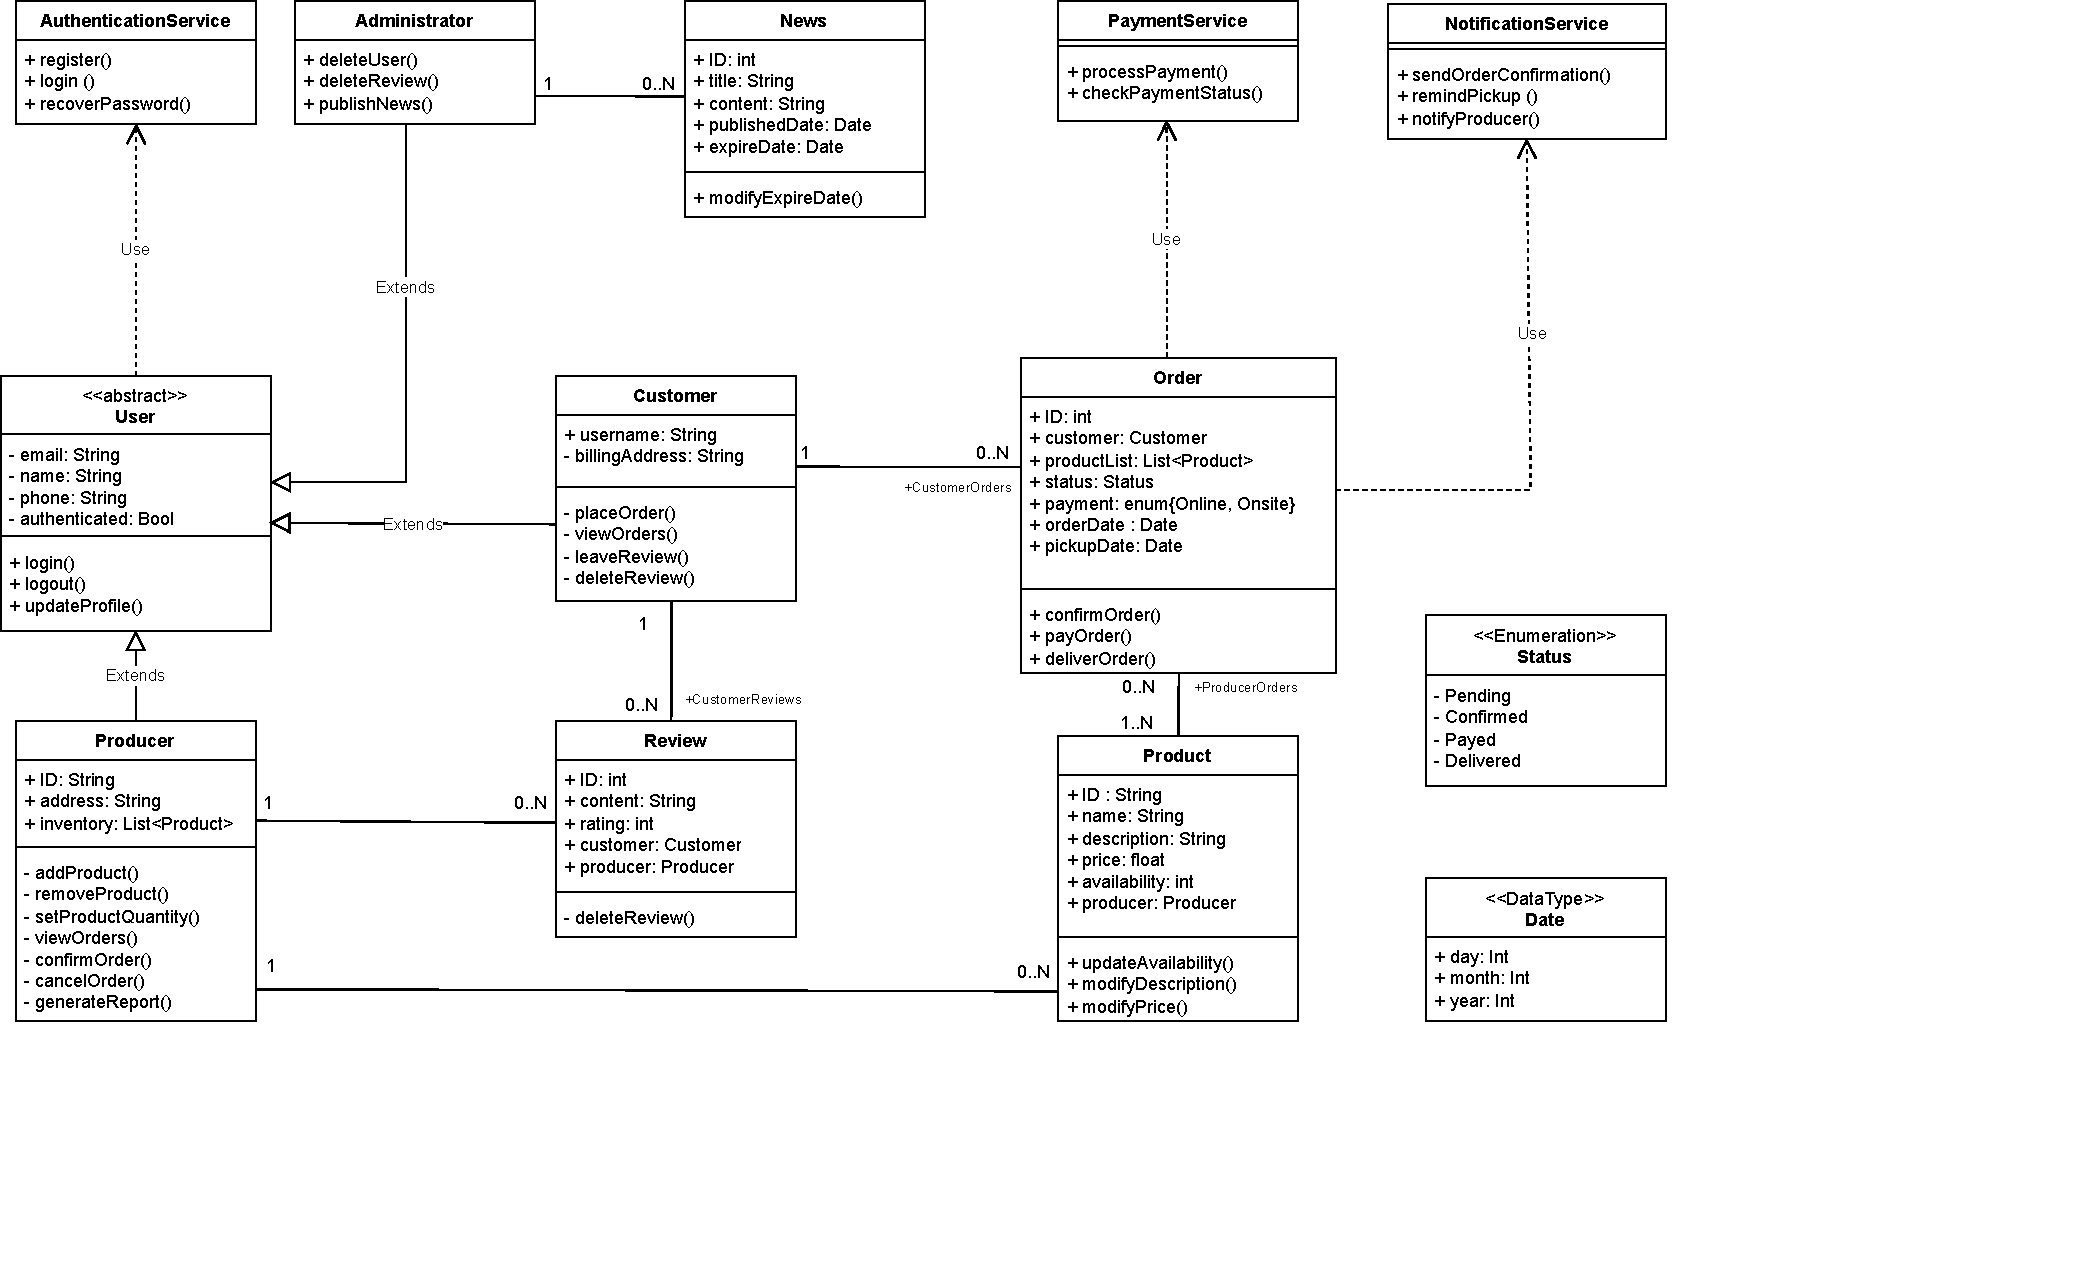
\includegraphics[trim= 0cm 4.3cm 7.3cm 0cm, clip, width=0.97\linewidth]{Deliverables/second-deliverable/img/Class-Diagram.drawio.pdf}
    \caption{Class Diagram}
\end{figure}

\end{landscape}

\restoregeometry

\newpage

\section{Diagramma delle classi}
\subsection{Classi di supporto}

\begin{itemize}
    \item \textbf{Date}: DataType che contiene gli attributi per descrivere i giorni dell'anno.
    
    \item \textbf{Status}: Enumerazione con i possibili stati di un ordine (Pending, Confirmed, Payed, Delivered).
\end{itemize}

\subsection{Autenticazione e profili utente}
\begin{itemize}
    \item \textbf{Authentication Service}:
Classe che si occupa della gestione del login, della registrazione e del recupero della password dell’utente appoggiandosi ad un servizio esterno.
\begin{table}[!htbp]
    \centering
    \begin{tabularx}{0.9\textwidth}{ >{\centering\arraybackslash}>{\centering\arraybackslash}m{4cm} | X }
    \hline
         \textbf{Operazione} & \textbf{Descrizione}\\
         \hline
         register() & legge i valori immessi in input dall’utente e lo registra tramite il servizio esterno di gestione account. Al termine della registrazione l’utente sarà automaticamente autenticato come Customer o Producer e l'attributo \texttt{authenticated} sarà impostato a \texttt{True}.\\
         \hline
         login() & verifica che i valori immessi (in particolare email e password) corrispondano con quelli effettivamente registrati dall’utente tramite servizio esterno. In caso di successo, imposterà il valore dell’attributo \texttt{authenticated} a  \texttt{True}.\\
         \hline
         recoverPassword() & legge l’email immessa dall’utente e richiede al servizio esterno di avviare la procedura per recuperare la password.\\
         \hline
    \end{tabularx}
    \caption{Authentication Service}
\end{table}

\item \textbf{User}: Classe astratta che rappresenta un utente del sistema. Contiene gli attributi comuni a tutti gli utenti, come email, password, e stato di autenticazione. È la base da cui derivano le classi specifiche per ogni tipo di utente (Customer, Producer, Administrator). 
\begin{table}[!htbp] 
    \centering 
    \begin{tabularx}{0.9\textwidth}{ >{\centering\arraybackslash}m{4cm} | X  }  
    \hline 
    \textbf{Operazione} & \textbf{Descrizione}\\
    \hline 
    login() & Richiama il servizio esterno ed esegue il login.\\ 
    \hline 
    logout() & Disconnette l'utente, impostando l'attributo \texttt{authenticated} a \texttt{False}.\\
    \hline 
    updateProfile() & Permette all'utente di aggiornare i propri dati.\\
    \hline 
    \end{tabularx} 
    \caption{User}
\end{table} 

\item \textbf{Administrator}:
Classe che rappresenta un amministratore del sistema. L'amministratore ha privilegi di gestione per l'intero sistema, inclusi la gestione degli utenti, delle recensioni e la pubblicazione di notizie.
\begin{table}[!htbp]
    \centering
    \begin{tabularx}{0.9\textwidth}{ >{\centering\arraybackslash}m{4cm} | X  } 
    \hline
         \textbf{Operazione} & \textbf{Descrizione} \\
         \hline
         deleteUser() & Consente all'amministratore di eliminare un utente dal sistema, sia esso un cliente o un produttore. \\
         \hline
         deleteReview() & Permette all'amministratore di eliminare una recensione lasciata da un cliente. \\
         \hline
         publishNews() & Consente all'amministratore di pubblicare notizie o aggiornamenti nel sistema, visibili a tutti gli utenti. \\
         \hline
    \end{tabularx}
    \caption{Administrator}
\end{table}

\item \textbf{Customer}:
Classe che rappresenta un cliente registrato nel sistema. Il cliente può fare ordini, visualizzare gli ordini precedenti, lasciare recensioni sui produttori e gestire i propri dati di pagamento.
\begin{table}[!htbp]
    \centering
    \begin{tabularx}{0.9\textwidth}{ >{\centering\arraybackslash}m{4cm} | X  } 
    \hline
         \textbf{Operazione} & \textbf{Descrizione} \\
         \hline
         placeOrder() & Consente al cliente di effettuare un ordine di uno o più prodotti. L'ordine viene registrato nel sistema e associato al cliente. \\
         \hline
         viewOrders() & Permette al cliente di visualizzare una lista dei propri ordini passati, con informazioni relative ai prodotti ordinati e allo stato dell'ordine. \\
         \hline
         leaveReview() & Permette al cliente di lasciare una recensione ad un produttore presso il quale ha concluso un acquisto. La recensione include una valutazione e un commento. \\
         \hline
         deleteReview() & Permette al cliente di eliminare una recensione precedentemente lasciata per un produttore. \\
         \hline
    \end{tabularx}
    \caption{Customer}
\end{table}


\item \textbf{Producer}:
Classe che rappresenta un produttore (azienda agricola) nel sistema. Il produttore è responsabile della gestione del proprio inventario di prodotti, della visualizzazione e gestione degli ordini, e della generazione di report.
\begin{table}[!htbp]
    \centering
    \begin{tabularx}{0.9\textwidth}{ >{\centering\arraybackslash}m{4cm} | X  } 
    \hline
         \textbf{Operazione} & \textbf{Descrizione} \\
         \hline
         addProduct() & Consente al produttore di aggiungere un nuovo prodotto al proprio inventario. Il prodotto viene registrato nel sistema con tutte le sue informazioni. \\
         \hline
         removeProduct() & Permette al produttore di rimuovere un prodotto dal proprio inventario. Il prodotto non sarà più disponibile per gli utenti. \\
         \hline
         setProductQuantity() & Consente al produttore o al sistema di aggiornare la quantità disponibile di un prodotto nell'inventario, in base alla disponibilità reale. \\
         \hline
         viewOrders() & Permette al produttore di visualizzare gli ordini ricevuti, con i dettagli relativi ai prodotti ordinati e allo stato dell'ordine. \\
         \hline
         confirmOrder() & Consente al produttore di confermare un ordine ricevuto, procedendo con la preparazione e spedizione dei prodotti. \\
         \hline
         cancelOrder() & Permette al produttore di annullare un ordine, per esempio se un prodotto non è disponibile o per altri motivi. \\
         \hline
         generateReport() & Consente al produttore di generare report sulle vendite, sugli ordini e sull'inventario, per monitorare le attività dell'azienda. \\
         \hline
    \end{tabularx}
    \caption{Producer}
\end{table}

\end{itemize}

\newpage
\subsection{Gestione ordine}
\begin{itemize}
    \item \textbf{Product}:
Classe che rappresenta un prodotto nel sistema. Ogni prodotto ha un identificatore, un nome, una descrizione, un prezzo, una quantità disponibile e un produttore associato. I prodotti sono gestiti dai produttori attraverso varie operazioni.
\begin{table}[!htbp]
    \centering
    \begin{tabularx}{0.9\textwidth}{ >{\centering\arraybackslash}m{4cm} | X  } 
    \hline
         \textbf{Operazione} & \textbf{Descrizione} \\
         \hline
         updateAvailability() & Consente al produttore di aggiornare la quantità disponibile del prodotto, in base alla disponibilità reale. \\
         \hline
         modifyDescription() & Permette al produttore di modificare la descrizione di un prodotto, ad esempio per aggiornare le informazioni o aggiungere dettagli. \\
         \hline
         modifyPrice() & Permette al produttore di modificare il prezzo di un prodotto. \\
         \hline
    \end{tabularx}
    \caption{Product}
\end{table}


\item \textbf{Order}:
Classe che rappresenta un ordine effettuato da un cliente nel sistema. Ogni ordine contiene un elenco di prodotti, lo stato dell'ordine, il metodo di pagamento, e le date relative all'ordine e al ritiro. L'ordine è associato a un cliente e può essere non confermato, confermato, pagato e consegnato.
\begin{table}[!htbp]
    \centering
    \begin{tabularx}{0.9\textwidth}{ >{\centering\arraybackslash}m{4cm} | X  } 
    \hline
         \textbf{Operazione} & \textbf{Descrizione} \\
         \hline
         confirmOrder() & Consente al cliente di confermare l'ordine, finalizzando la selezione dei prodotti e inoltrando la richiesta al produttore. \\
         \hline
         payOrder() & Permette al cliente di effettuare il pagamento dell'ordine, che può essere online o sul posto, a seconda del metodo di pagamento selezionato. \\
         \hline
         deliverOrder() & Consente al produttore di segnare l'ordine come consegnato, completando così il processo di acquisto. \\
         \hline
    \end{tabularx}
    \caption{Order}
\end{table}


\item \textbf{Review}:
Classe che rappresenta una recensione lasciata da un cliente su un produttore. Ogni recensione contiene un contenuto testuale, una valutazione numerica, e i riferimenti al cliente e al produttore. Le recensioni possono essere rimosse, se necessario.
\begin{table}[!htbp]
    \centering
    \begin{tabularx}{0.9\textwidth}{ >{\centering\arraybackslash}m{4cm} | X  } 
    \hline
         \textbf{Operazione} & \textbf{Descrizione} \\
         \hline
         deleteReview() & Permette al cliente di eliminare una recensione precedentemente lasciata al produttore. \\
         \hline
    \end{tabularx}
    \caption{Review}
\end{table}

\end{itemize}

\newpage
\subsection{Altre classi e servizi}

\begin{itemize}
    \item \textbf{News}:
Classe che rappresenta una notizia pubblicata nel sistema. Ogni notizia contiene un titolo, un contenuto, una data di pubblicazione e una data di scadenza. Le notizie possono essere modificate, in particolare per quanto riguarda la data di scadenza.
\begin{table}[!htbp]
    \centering
    \begin{tabularx}{0.9\textwidth}{ >{\centering\arraybackslash}m{4cm} | X  } 
    \hline
         \textbf{Operazione} & \textbf{Descrizione} \\
         \hline
         modifyExpireDate() & Consente all'amministratore di modificare la data di scadenza di una notizia, prolungando o accorciando la sua visibilità nel sistema. \\
         \hline
    \end{tabularx}
    \caption{News}
\end{table}


\item \textbf{PaymentService}:
Classe che gestisce l'elaborazione dei pagamenti per gli ordini. Si occupa di processare i pagamenti e di verificare lo stato delle transazioni. È utilizzato dal sistema per completare il pagamento degli ordini effettuati dai clienti.
\begin{table}[!htbp]
    \centering
    \begin{tabularx}{0.9\textwidth}{ >{\centering\arraybackslash}m{4cm} | X  } 
    \hline
         \textbf{Operazione} & \textbf{Descrizione} \\
         \hline
         processPayment() & Gestisce il pagamento di un ordine, interagendo con il sistema di pagamento esterno per completare la transazione. \\
         \hline
         checkPaymentStatus() & Verifica lo stato di un pagamento effettuato, restituendo informazioni sulla riuscita o meno della transazione. \\
         \hline
    \end{tabularx}
    \caption{PaymentService}
\end{table}

\item \textbf{NotificationService}:
Classe che gestisce l'invio delle notifiche agli utenti del sistema. Si occupa di inviare conferme degli ordini, promemoria per il ritiro e notifiche ai produttori riguardo agli ordini ricevuti o altre attività rilevanti.
\begin{table}[!htbp]
    \centering
    \begin{tabularx}{0.9\textwidth}{ >{\centering\arraybackslash}m{4cm} | X  } 
    \hline
         \textbf{Operazione} & \textbf{Descrizione} \\
         \hline
         sendOrderConfirmation() & Invia una notifica di conferma al cliente dopo che un ordine è stato effettuato, includendo i dettagli dell'ordine. \\
         \hline
         remindPickup() & Invia un promemoria al cliente riguardo la data di ritiro dell'ordine, per assicurarsi che il cliente non dimentichi di ritirarlo. \\
         \hline
         notifyProducer() & Invia una notifica al produttore riguardo un nuovo ordine ricevuto, inclusi i dettagli sui prodotti ordinati e la data di ritiro. \\
         \hline
    \end{tabularx}
    \caption{NotificationService}
\end{table}

\end{itemize}